\section{Motivation}
\label{sec:moti}
The original \cb{} 

\subsection{The architecture of the original \cb{}}
The user's browser will download the client engine written in javascript.
The client engine then connect to the server and fetch DOM elements in a
virtual browser
will connect to a virtual browser in server side and fetch DOM
elements from the 

The requests are translated to DOM events by the framework to be triggered on virtual browsers.
The application javascript code would handle these events and update the DOM elements.
Finally the 

\begin{figure}[h!]
\centering
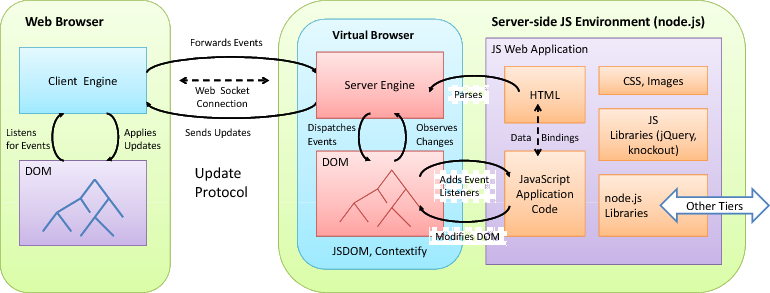
\includegraphics[width=\textwidth]{figs/cb1_architecture_overview}
\caption{Single Process \cb{} Architecture Overview}
\label{fig:cb1arch}
\end{figure}
